\documentclass[12pt,a4paper,UTF8]{article}

\usepackage[titletoc]{appendix}
\usepackage{xeCJK}
\usepackage{amsmath}
\usepackage{array}
\usepackage{bm}
\usepackage{booktabs}
\usepackage{caption}
\usepackage{cite}
\usepackage{comment}
\usepackage{float}
\usepackage{fontspec} % xelatex限定
\usepackage{geometry}
\usepackage{graphicx}
\usepackage{indentfirst}
% \usepackage[utf8]{inputenc} % 非xelatex编译,显式指定文件编码为utf8
\usepackage{listings}
\usepackage{longtable}
\usepackage{mathtools}
\usepackage{multicol}
\usepackage{multirow}
\usepackage{supertabular}
\usepackage{subcaption}
\usepackage{tabu}
\usepackage{ulem}
\usepackage{url}
\usepackage{xcolor}
\usepackage{nccmath} % だが align* は nccmath が無くても使えるので敢えて両方書いた。
% \usepackage{CJKutf8}
% \usepackage{hyperref}

\geometry{a4paper,left=2.5cm,right=2.5cm,top=2.5cm,bottom=2.5cm}
\defaultCJKfontfeatures{Scale=1.2}
\linespread{1.5}

%% Define a new 'leo' style for the package that will use a smaller font.
\makeatletter
\def\url@leostyle{%
  \@ifundefined{selectfont}{\def\UrlFont{\sf}}{\def\UrlFont{\small\ttfamily}}}
\makeatother
\urlstyle{leo} % Now actually use the newly defined style.


\renewcommand{\contentsname}{\centering{目录}}
\renewcommand{\abstractname}{\large{摘要}}
\def\tablename{表}
\def\figurename{图}
\renewcommand{\thetable}{\thesection.\arabic{table}}
\renewcommand{\thefigure}{\thesection.\arabic{figure}}
\renewcommand{\multirowsetup}{\centering}
\renewcommand{\appendixname}{附录~\Alpha{section}}
\renewcommand{\refname}{参考文献}

\everymath{\displaystyle}
\bibliographystyle{plain}


\lstdefinestyle{BASH}{
    breaklines=true,                                     % 自动换行
    columns=fixed,
    extendedchars=true,                                  % lets you use non-ASCII characters; for 8-bits encodings only, does not work with UTF-8
    frame=shadowbox,                                     % 设置背景边框
    numbers=left,                                        % 在左侧显示行号
    numberstyle=\footnotesize\color{darkgray},           % 设定行号格式
    showstringspaces=false,                              % 不显示字符串中的空格
    tabsize=4,	                                         % 设置tab长度
}
\lstdefinestyle{tinyBASH}{
    breaklines=true,                                     % 自动换行
    basicstyle=\footnotesize\ttfamily,
    columns=fixed,
    extendedchars=true,                                  % lets you use non-ASCII characters; for 8-bits encodings only, does not work with UTF-8
    frame=shadowbox,                                     % 设置背景边框
    numbers=left,                                        % 在左侧显示行号
    numberstyle=\footnotesize\color{darkgray},           % 设定行号格式
    showstringspaces=false,                              % 不显示字符串中的空格
    tabsize=4,	                                         % 设置tab长度
}
\lstdefinestyle{Python}{
    breaklines=true,                                     % 自动换行
    captionpos=b,                                        % sets the caption-position to bottom
    columns=fixed,
    commentstyle=\it\color[RGB]{0,96,96},                % 设置代码注释的格式
    % extendedchars=true,                                  % lets you use non-ASCII characters; for 8-bits encodings only, does not work with UTF-8
    frame=shadowbox,                                     % 设置背景边框
    keywordstyle=\bfseries\color[RGB]{40,40,255},        % 设定关键字颜色
    language=Python,                                     % 设置语言
    numbers=left,                                        % 在左侧显示行号
    numberstyle=\footnotesize\color{darkgray},           % 设定行号格式
    stringstyle=\rmfamily\slshape\color[RGB]{128,0,0},   % 设置字符串格式
    tabsize=4,	                                         % 设置tab长度
}

\lstdefinestyle{CPP}{
    %backgroundcolor=\color[RGB]{245,245,244},           % 设定背景颜色
    breaklines=true,                                     % 自动换行
    captionpos=b,                                        % sets the caption-position to bottom
    columns=fixed,
    commentstyle=\it\color[RGB]{0,96,96},                % 设置代码注释的格式
    extendedchars=true,                                  % lets you use non-ASCII characters; for 8-bits encodings only, does not work with UTF-8
    frame=shadowbox,                                     % 设置背景边框
    keywordstyle=\bfseries\color[RGB]{40,40,255},        % 设定关键字颜色
    language=c++,                                        % 设置语言
    numbers=left,                                        % 在左侧显示行号
    numberstyle=\footnotesize\color{darkgray},           % 设定行号格式
    showstringspaces=false,                              % 不显示字符串中的空格
    stringstyle=\rmfamily\slshape\color[RGB]{128,0,0},   % 设置字符串格式
    tabsize=4,	                                         % 设置tab长度
    title=\lstname,                                      % show the filename of files included with \lstinputlisting; also try caption instead of title
    morekeywords={alignas,continute,friend,register,true,alignof,decltype,goto,
        reinterpret_cast,try,asm,defult,if,return,typedef,auto,delete,inline,short,
        typeid,bool,do,int,signed,typename,break,double,long,sizeof,union,case,
        dynamic_cast,mutable,static,unsigned,catch,else,namespace,static_assert,using,
        char,enum,new,static_cast,virtual,char16_t,char32_t,explict,noexcept,struct,
        void,export,nullptr,switch,volatile,class,extern,operator,template,wchar_t,
        const,false,private,this,while,constexpr,float,protected,thread_local,
        const_cast,for,public,throw,std},
    emph={map,set,multimap,multiset,unordered_map,unordered_set,
        unordered_multiset,unordered_multimap,vector,string,list,deque,
        array,stack,forwared_list,iostream,memory,shared_ptr,unique_ptr,
        random,bitset,ostream,istream,cout,cin,endl,move,default_random_engine,
        uniform_int_distribution,iterator,algorithm,functional,bing,numeric},
}

\lstdefinestyle{QT}{
    %backgroundcolor=\color[RGB]{245,245,244},           % 设定背景颜色
    breaklines=true,                                     % 自动换行
    captionpos=b,                                        % sets the caption-position to bottom
    columns=fixed,
    commentstyle=\it\color[RGB]{0,96,96},                % 设置代码注释的格式
    extendedchars=true,                                  % lets you use non-ASCII characters; for 8-bits encodings only, does not work with UTF-8
    frame=shadowbox,                                     % 设置背景边框
    keywordstyle=\bfseries\color[RGB]{40,40,255},        % 设定关键字颜色
    language=c++,                                        % 设置语言
    numbers=left,                                        % 在左侧显示行号
    numberstyle=\footnotesize\color{darkgray},           % 设定行号格式
    stringstyle=\rmfamily\slshape\color[RGB]{128,0,0},   % 设置字符串格式
    showstringspaces=false,                              % 不显示字符串中的空格
    tabsize=4,	                                         % 设置tab长度
    title=\lstname,                                      % show the filename of files included with \lstinputlisting; also try caption instead of title
    morekeywords={alignas,continute,friend,register,true,alignof,decltype,goto,
        reinterpret_cast,try,asm,defult,if,return,typedef,auto,delete,inline,short,
        typeid,bool,do,int,signed,typename,break,double,long,sizeof,union,case,
        dynamic_cast,mutable,static,unsigned,catch,else,namespace,static_assert,using,
        char,enum,new,static_cast,virtual,char16_t,char32_t,explict,noexcept,struct,
        void,export,nullptr,switch,volatile,class,extern,operator,template,wchar_t,
        const,false,private,this,while,constexpr,float,protected,thread_local,
        const_cast,for,public,throw,std,bind,function,
        Q_OBJECT,QDialog,QUdpSocket,QTcpSocket,QHostAddress,QNetworkDatagram,QTcpServer,
        QByteArray,QString,QStringList,QList,QSet,QMap,
        quint,qint64,uintptr_t,
        connect,signals,slots,SIGNAL,SLOT},
    emph={map,set,multimap,multiset,unordered_map,unordered_set,
        unordered_multiset,unordered_multimap,vector,string,list,deque,
        array,stack,forwared_list,iostream,memory,shared_ptr,unique_ptr,
        random,bitset,ostream,istream,cout,cin,endl,move,default_random_engine,
        uniform_int_distribution,iterator,algorithm,functional,bing,numeric},
}

\lstdefinestyle{MASM}{
    breaklines=true,                                     % 自动换行
    captionpos=b,                                        % sets the caption-position to bottom
    columns=fixed,
    commentstyle=\it\color[RGB]{0,96,96},                % 设置代码注释的格式
    extendedchars=true,                                  % lets you use non-ASCII characters; for 8-bits encodings only, does not work with UTF-8    
    frame=shadowbox,                                     % 设置背景边框
    keywordstyle=\bfseries\color[RGB]{40,40,255},        % 设定关键字颜色
    language=[x86masm]Assembler,                         % 设置语言
    numbers=left,                                        % 在左侧显示行号
    numberstyle=\footnotesize\color{darkgray},           % 设定行号格式
    stringstyle=\rmfamily\slshape\color[RGB]{128,0,0},   % 设置字符串格式
    showstringspaces=false,                              % 不显示字符串中的空格
    tabsize=4,	                                         % 设置tab长度
    title=\lstname,                                      % show the filename of files included with \lstinputlisting; also try caption instead of title
    morekeywords={CDQE,CQO,CMPSQ,CMPXCHG16B,JRCXZ,LODSQ,MOVSXD, % 
        POPFQ,PUSHFQ,SCASQ,STOSQ,IRETQ,RDTSCP,SWAPGS, % 
        .code,.def,.file,.type,.ended,.scl,.section,.ascii,.text,.globl,.ident,.rodata,
        .sch_proc,.sch_pushreg,.sch_setframe,.sch_stackalloc,.sch_endprologue,.sch_endproc,
        pushq,popq,movq,movl,addq,subq,leaq,invoke,start,addr,
        rax,rdx,rcx,rbx,rsi,rdi,rip,rsp,rbp, % 
        r8,r8d,r8w,r8b,r9,r9d,r9w,r9b, % 
        r10,r10d,r10w,r10b,r11,r11d,r11w,r11b, % 
        r12,r12d,r12w,r12b,r13,r13d,r13w,r13b, % 
        r14,r14d,r14w,r14b,r15,r15d,r15w,r15b}
}
\newcommand{\includecode}[2][c]{\lstinputlisting[caption=#2, escapechar=, style=#1]{#2}}



% \setcounter{table}{0}
% \setcounter{figure}{0}

% \lstinputlisting[style=CPP]{src/main.cpp}

% \begin{figure}[H]
%     \centering
%     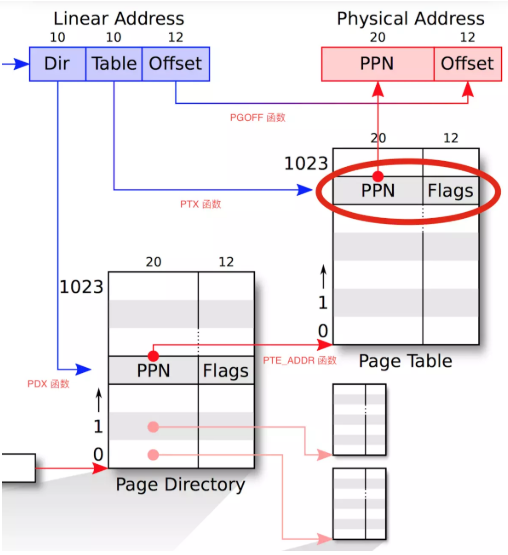
\includegraphics[width = .75\linewidth]{img/1.png}
%     \caption{预处理结果(部分)}
%     \label{fig::figure2}
% \end{figure}


% 结果如表\ref{tab::table2}:
% \begin{table}[htbp]
%     \begin{center}
%         \begin{tabular}{c c c}
%             \toprule
%             优化等级 & 二进制文件大小(Byte) &  执行时间(s)\\
%             \midrule
%             不优化 & 13992 & 36.090 \\
%             O1 & 13344 & 10.562\\
%             O2 & 13344 & 9.925\\
%             Os & 13344 & 8.899\\
%             O3 & 13344 & 8.350\\
%             Ofast & 14800 & 8.094\\
%             \bottomrule
%         \end{tabular}
%         \caption{各等级优化测试结果}\label{tab::table2}
%     \end{center}
% \end{table}

% \begin{equation}
%     \begin{split}
%         id     & \rightarrow char\ |\ id\ digit\ |\ id\ char \\
%         digit  & \rightarrow 0\ |\ 1\ |\ 2\ |\ 3\ |\ 4\ |\ 5\ |\ 6\ |\ 7\ |\ 8\ |\ 9 \\
%         char   & \rightarrow \_\ |\ letter \\
%         letter & \rightarrow A\ |\ B\ |\ ...\ |\ Z\ |\ a\ |\ b\ |\ ...\ |\ z \\
%     \end{split}
% \end{equation}


\begin{document}

\title{Lab 2: Memory Management}
\author{\ }
\date{\today}

\maketitle

\begin{abstract}
    \setlength{\parindent}{2em}
    本次实验取自MIT\ 6.828\ Lab2,共分为三个部分。第一部分学习并编写物理页面管理。
    第二部分学习并修改虚拟内存相关组件。第三部分学习内存地址空间。

    \textbf{关键词:JOS、内存页面、虚拟内存}
\end{abstract}

\section{作业三}

    \subsection{boot\_alloc()}
    用来申请n个字节的空间(会被4K对齐),返回申请好的空间的首地址,如果n==0,则返回当前未分配的空间的首地址。

    \begin{lstlisting}[style=CPP]
static void *
boot_alloc(uint32_t n)
{
	static char *nextfree;
	char *result;

	if (!nextfree) {
		extern char end[];
		nextfree = ROUNDUP((char*)end, PGSIZE);
	}
	if(n==0)
		return nextfree;
	result = nextfree;
	nextfree += n;
	nextfree = ROUNDUP((char*)nextfree, PGSIZE);
	return result;
}
    \end{lstlisting}

    这里,end代表bss段的末尾,即当前未分配空间的首部;ROUNDUP函数实现向上取整倍数,用来4K对齐。
    
    当n$>$0时,先将nextfree,即当前未分配空间的首地址赋值给result,再将nextfree向后加4K对齐的n个字节,
    这时result就是申请好的空间的首地址。

    \subsection{mem\_init()}

    大部分函数都在这个函数里被调用,需要添加的是为pages申请空间并初始化的代码。代码如下:

    \begin{lstlisting}[style=CPP]
pages = boot_alloc(npages * sizeof (struct PageInfo));
memset(pages, 0, npages * sizeof(struct PageInfo));
    \end{lstlisting}

    这里boot\_alloc()的参数是页数乘每页大小(结构体而非实际页),正好是需要申请的空间大小。

    \subsection{page\_init()}
    负责page结构体和内存空闲链表的初始化。根据注释的要求实现代码如下:

    \begin{lstlisting}[style=CPP]
void
page_init(void)
{
	size_t i;
	for (i = 0; i < npages; i++) {
		if(i == 0) {	
            pages[i].pp_ref = 1;
			pages[i].pp_link = NULL;
		} else if (i >= 1 && i < npages_basemem) {
			pages[i].pp_ref = 0;
			pages[i].pp_link = page_free_list; 
			page_free_list = &pages[i];
		} else if (i >= IOPHYSMEM / PGSIZE && i < EXTPHYSMEM/PGSIZE) {
			pages[i].pp_ref = 1;
			pages[i].pp_link = NULL;
        } else if (i >= EXTPHYSMEM / PGSIZE && 
                   i < ((int)(boot_alloc(0)) - KERNBASE) / PGSIZE) {
			pages[i].pp_ref = 1;
			pages[i].pp_link =NULL;
		} else {
			pages[i].pp_ref = 0;
			pages[i].pp_link = page_free_list;
			page_free_list = &pages[i];
		}
	}
}
    \end{lstlisting}

    这里的pages是PageInfo结构体数组,PageInfo有两个成员:struct PageInfo *pp\_link 和 uint16\_t pp\_ref,
    pp\_ref指出当前页的被引次数,pp\_link指向下一个空闲页。


    进行初始化时,当这个页是空闲页时,前者指向下一个空闲页,否则为空。
    即所有空闲页通过链表连接在一起,占用页则没有联系;
    但事实上全部的页(空闲页,占用页)相邻地分布在boot\_alloc函数所申请的空间里,并通过指针进行访问。
    同时,需要保证第一个对象的pp\_link为空,空闲页的pp\_ref置0、占用页置1,以及page\_free\_list永远指向表头。

    \subsection{page\_alloc()}

    这个函数是为了分配一个物理页,
    如果当前有空闲的页,那么将其返回,并且找到下一个空闲的页。

    \begin{lstlisting}[style=CPP]
struct PageInfo *
page_alloc(int alloc_flags)
{	
    if (page_free_list == NULL)
		return NULL;
	struct PageInfo* page = page_free_list;
	page_free_list = page->pp_link;
	page->pp_link = 0;
	if (alloc_flags & ALLOC_ZERO)
		memset(page2kva(page), 0, PGSIZE);
	return page;
}
    \end{lstlisting}

    我们将表头,也就是page\_free\_list指向的对象从链表上取出(pp\_link置0)并分配,在需要的情况下将新分配的页置0。

    \subsection{page\_free()}

    该函数释放一个页,当pp\_ref不为0(页面仍被使用)时,以及当pp\_link不为空(页面已经被释放)时,需要提出panic。

    \begin{lstlisting}[style=CPP]
void
page_free(struct PageInfo *pp)
{
    if (pp->pp_ref != 0)
        panic("This page is still been used.")
    if (pp->pp_link != 0) 
		panic("This page has been freed");
	pp->pp_link = page_free_list;
	page_free_list = pp;
	return; 
}
    \end{lstlisting}


\section{问题三}

x是uintptr\_t类型。

因为这里变量value使用了$*$操作符解析地址,即先转为指针再解析引用的方式,是虚拟地址。
所以变量x也应该是虚拟地址也就是uintptr\_t类型。

\section{作业四}
\setcounter{table}{0}
\setcounter{figure}{0}

    为了补全代码,需要了解以下两个宏:

    \begin{lstlisting}[style=CPP]
#define PADDR(kva) _paddr(__FILE__, __LINE__, kva)
#define KADDR(pa) _kaddr(__FILE__, __LINE__, pa)
    \end{lstlisting}

    PADDR()接受一个内核虚拟地址,并返回相应的物理地址;KADDR()接受一个物理地址并返回相应的内核虚拟地址。
    由于JOS将物理地址0映射到虚拟地址0xf0000000,因此两个宏实际的操作是将地址加上或减去这个数。

    \subsection{pgdir\_walk()}

    pgdir\_walk()用于查找虚拟地址对应的页表项地址,
    传入参数分别为页目录项指针、线性地址和一个用于判断页目录项不存在时是否进行创建参数。
    返回值为页表项指针,在页表不存在且create==false或创建页表失败时,返回NULL。
    
    查找页表项地址之前首先要获得页目录地址,对页表是否存在进行判断,
    如果页目录存在,直接进行映射;如果不存在,则新建一个页表后再进行映射。
    创建页表时使用page\_alloc分配新的页表页,并为新建的物理页设置页目录时添加上权限位。查找过程如下图\ref{fig::figure1}:

    \begin{figure}[H]
        \centering
        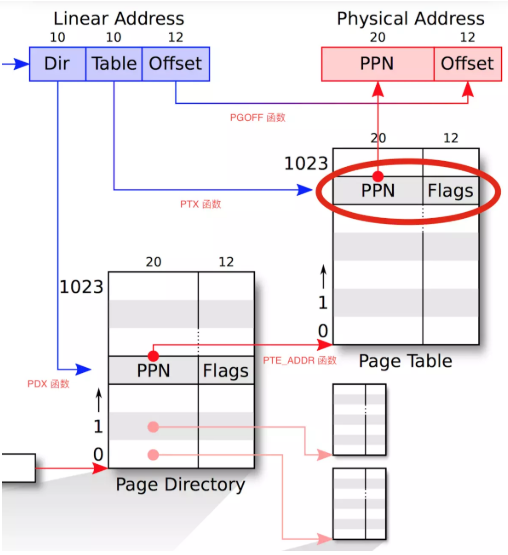
\includegraphics[width = .75\linewidth]{img/1.png}
        \caption{查找过程}
        \label{fig::figure1}
    \end{figure}

    具体代码如下:

    \begin{lstlisting}[style=CPP]
pte_t *
pgdir_walk(pde_t *pgdir, const void *va, int create)
{
	// Fill this function in
	pde_t *pt = pgdir + PDX(va);
   	pde_t *pt_addr_v;

    if (*pt & PTE_P) {
   	   pt_addr_v = (pte_t*)KADDR(PTE_ADDR(*pt));
   	   return pt_addr_v + PTX(va);
   	} else {
	    struct PageInfo *newpt = page_alloc(ALLOC_ZERO);
        if (create == 1 && newpt != 0) {
            memset(page2kva(newpt), 0, PGSIZE);
            newpt->pp_ref ++;
            *pt = PADDR(page2kva(newpt)) | PTE_U | PTE_W | PTE_P;
            pt_addr_v = (pte_t*)KADDR(PTE_ADDR(*pt));
            return pt_addr_v + PTX(va);
        }
    }
	return NULL;
}
    \end{lstlisting}

    \subsection{boot\_map\_region()}

    boot\_map\_region()将虚拟地址[va, va+size)映射到物理地址[pa, pa+size),
    传入参数中,size是PGSIZE的倍数,va和pa都是page-aligned。
    
    反复调用pgdir\_walk,获取页表地址,其中va类型是uintptr\_t,
    调用pgdir\_walk时需要将其转换为void*,并对获取到的页表地址使用权限位perm$|$PTE\_P。

    具体代码如下:
    \begin{lstlisting}[style=CPP]
static void
boot_map_region(pde_t *pgdir, uintptr_t va, size_t size, physaddr_t pa, int perm)
{
	int offset;
    pte_t *pt;
    for (offset = 0; offset < size; offset += PGSIZE) {
        pt = pgdir_walk(pgdir, (void*)va, 1);
        *pt = pa|perm|PTE_P;
        pa += PGSIZE;
        va += PGSIZE;
   	}
}
    \end{lstlisting}

    \subsection{page\_lookup()}

    page\_lookup()用于查找线性地址va对应的物理页面,找到就返回这个物理页,否则返回NULL。
    参数为页目录指针、线性地址和指向页表指针的指针。

    利用pgdir\_walk()查找va对应的物理页面,如果pte\_store不为零,则在其中存储此页的pte地址。

    具体代码如下:
    \begin{lstlisting}[style=CPP]
struct PageInfo *
page_lookup(pde_t *pgdir, void *va, pte_t **pte_store)
{
	pte_t *pte = pgdir_walk(pgdir, va, 0);
   	if (pte_store != 0) {
        *pte_store = pte;
   	}
   	if (pte != NULL && (*pte & PTE_P)) {
      	return pa2page(PTE_ADDR(*pte));
   	}
	return NULL;
}
    \end{lstlisting}

    \subsection{page\_remove()}

    page\_remove()在虚拟地址“va”处取消对物理页面的映射,如果该地址没有物理页面,就什么都不做。
    
    通过page\_lookup获得物理页,如果物理页存在,利用page\_decref进行删除工作,
    然后将va地址的页表项设为0,并对有效性进行验证。
    
    具体代码如下:

    \begin{lstlisting}[style=CPP]
void
page_remove(pde_t *pgdir, void *va)
{
 	pte_t *pte;
    struct PageInfo *page = page_lookup(pgdir, va, &pte);
    if (page) {
        page_decref(page);
        *pte = 0;
        tlb_invalidate(pgdir, va);
    }
}
    \end{lstlisting}

    \subsection{page\_insert()}

    page\_insert()建立一个虚拟地址与物理页的映射,将页面管理结构pp所对应的物理页面分配给线性地址va。
    传入参数为页目录指针、页描述结构体指针、线性地址,和权限,建立映射成功,返回0,失败返回-E\_NO\_MEM(内存不足)

    利用pgdir\_walk()查找该虚拟地址对应的页表项,查找失败,返回-E\_NO\_MEM,
    否则,对查找结果进行判断,如果映射到与之前相同的物理页,应调用page\_remove删除之前的映射关系,重新建立映射。
    如果映射到与之前不同的物理页面,则将va对应的页表项中的物理地址重新赋值为pp所对应的物理页面的首地址。
    建立映射时应将对应的页表项的权限(低12位)设置成PTE\_P \& perm,插入成功,-pp-$>$pp\_ref递增。

    具体代码如下:

    \begin{lstlisting}[style=CPP]
int
page_insert(pde_t *pgdir, struct PageInfo *pp, void *va, int perm)
{
	pte_t *pte = pgdir_walk(pgdir, va, 1);
    if (!pte)
        return -E_NO_MEM;
   	if (*pte & PTE_P) {
        if (PTE_ADDR(*pte) == page2pa(pp)) {
           tlb_invalidate(pgdir, va);
           pp->pp_ref--;
        } else {
	        page_remove(pgdir, va);
  	    }
  	}
	*pte = page2pa(pp) | perm | PTE_P;
 	pp->pp_ref++;
  	pgdir[PDX(va)] |= perm;
	return 0;
}
    \end{lstlisting}

    对映射到的物理页进行区分会出一些问题,则不进行区分,直接删除之前的映射关系,对函数进行调整,代码如下:

    \begin{lstlisting}[style=CPP]
int 
page_insert(pde_t *pgdir, struct PageInfo *pp, void *va, int perm)
{
    pte_t *pte = pgdir_walk(pgdir, va, 1);
    if (!pte)
        return -E_NO_MEM;
    pp->pp_ref++;
    if (*pte & PTE_P)
        page_remove(pgdir, va);
    *pte = page2pa(pp) | perm | PTE_P;
    return 0;
}
    \end{lstlisting}


\section{作业五}

    按要求分别加入三处代码如下:
    \begin{lstlisting}[style=CPP]
boot_map_region(kern_pgdir, UPAGES, PTSIZE, PADDR(pages), PTE_U);

boot_map_region_large(kern_pgdir, KSTACKTOP-KSTKSIZE, KSTKSIZE, PADDR(bootstack), PTE_W);

boot_map_region(kern_pgdir, KERNBASE, -KERNBASE, 0, PTE_W);
    \end{lstlisting}

    从mem\_init()中的注释信息中,我们得知需使用boot\_map\_region()函数。

    boot\_map\_region()的作用是将一段连续的虚拟地址映射到它所对应的物理地址中。
    
    观察这个函数的参数:第一个是页面的目录,第二个是虚拟地址,第三是映射范围大小,第四是对应物理地址,第五是赋予的权限。

    第一部分的映射,起点是UPAGES,大小是PTSIZE,物理地址是PADDR(pages),
    权限是PTE\_U$|$PTE\_P ,这里不写PTE\_P是因为函数内部已经自己默认赋予此权限了。

    \begin{lstlisting}[style=CPP]
// UVPT   ----> +------------------------------+ 0xef400000
//              |          RO PAGES            | R-/R-  PTSIZE
// UPAGES ----> +------------------------------+ 0xef000000
//              |           RO ENVS            | R-/R-  PTSIZE
    \end{lstlisting}

    第二部分的映射,起点是KSTACKTOP-KSTKSIZE,大小是KSTKSIZE,物理地址是 PADDR(bootstack),
    权限是PTE\_W,这里不写PTE\_P是因为函数内部已经自己默认赋予此权限了。
    内核堆栈的虚拟地址范围是[KSTACKTOP-PTSIZE, KSTACKTOP),
    但是我们只把[KSTACKTOP-KSTKSIZE, KSTACKTOP)这部分映射关系加入到页表中,
    [KSTACKTOP-PTSIZE, KSTACKTOP-KSTKSIZE)这部分不进行映射。

    第三部分的映射,虚拟地址范围是[KERNBASE,4G],物理地址范围是[0,2\^32-KERNBASE]。权限是PTE\_W 。 

    \begin{lstlisting}[style=CPP]
// 4 Gig -------->  +------------------------------+
//                  |                              | RW/--
//                  ~~~~~~~~~~~~~~~~~~~~~~~~~~~~~~~~
//                  :              .               :
//                  :              .               :
//                  :              .               :
//                  |~~~~~~~~~~~~~~~~~~~~~~~~~~~~~~| RW/--
//                  |                              | RW/--
//                  |   Remapped Physical Memory   | RW/--
//                  |                              | RW/--
// KERNBASE, ---->  +------------------------------+ 0xf0000000
    \end{lstlisting}


\section{问题四}
    \subsection{第一问}
    假设下图描述的是系统的页目录表,哪些条目(行)已经被填充了?
    它们是怎么样进行地址映射的?它们所指向的位置在哪里?请尽可能完善这张表的内容。
    
    根据memlayout.h中的布局图,我们填写该表如下表\ref{tab::table2}:
    \begin{table}[htbp]
        \begin{center}
            \begin{tabular}{c c c}
                \toprule
                Entry & Base Virtual Address & Points to (logically) \\
                \midrule
                1023    &   0xffc0000   &   Page table for top 4MB of phys memory \\
                1022    &   0xff80000   &   ...... \\
                ...     &               &    \\
                960     &   0xf0000000	&	Page table for bottom 4MB of phys memory \\
                959     &   0xefc00000	&	Current page table, kernel RW \\
                958     &   0xef800000	&	Kernel stack \\
                957     &   0xef400000  &   Current page table kernel R-, user R- \\
                956	    &   0xef000000  &	User pages \\
                ...     &               &    \\
                2       &   0x00800000  &    \\
                1       &   0x00400000  &    \\
                0       &   0x00000000  &   Empty Memory \\
                \bottomrule
            \end{tabular}
            \caption{问题4-1}\label{tab::table2}
        \end{center}
    \end{table}

    \subsection{第二问}
    我们已经将内核和用户环境放在同一地址空间内。为什么用户的程序不能读取内核的内存?
    有什么具体的机制保护内核空间吗?
    
    因为虚拟内存被ULIM和UTOP划分为不同的段,(ULIM, 4GB)只允许内核读写,(UTOP, ULIM]只允许内核和用户读取,
    而[0x0, UTOP]允许内核与用户读写。

    我们通过在页(目录)表中设置保护位的机制来确保这点,包括PTE\_W(writeable)和PTE\_U(user)。

    \subsection{第三问}
    JOS最大支持多大的物理内存,为什么?

    4GB。因为页目录表一共包含了1024个指针,每个指向一个页表,
    而每个页表包含1024个指针,每个指向一个物理页面,其大小为4096bytes。
    因此总大小为$1024*1024*4096B=4GB$。
    
    \subsection{第四问}
    如果我们的硬件配置了可以支持的最大的物理内存,那么管理内存空间的开销是多少?
    这一开销是怎样划分的?

    易得sizeof PageInfo = 8 bytes,因此8MB用于页面信息,4MB用于页表,4KB用于页目录表。

\section{实验结果}

    执行make grade,得到结果如下:
    \begin{figure}[H]
        \centering
        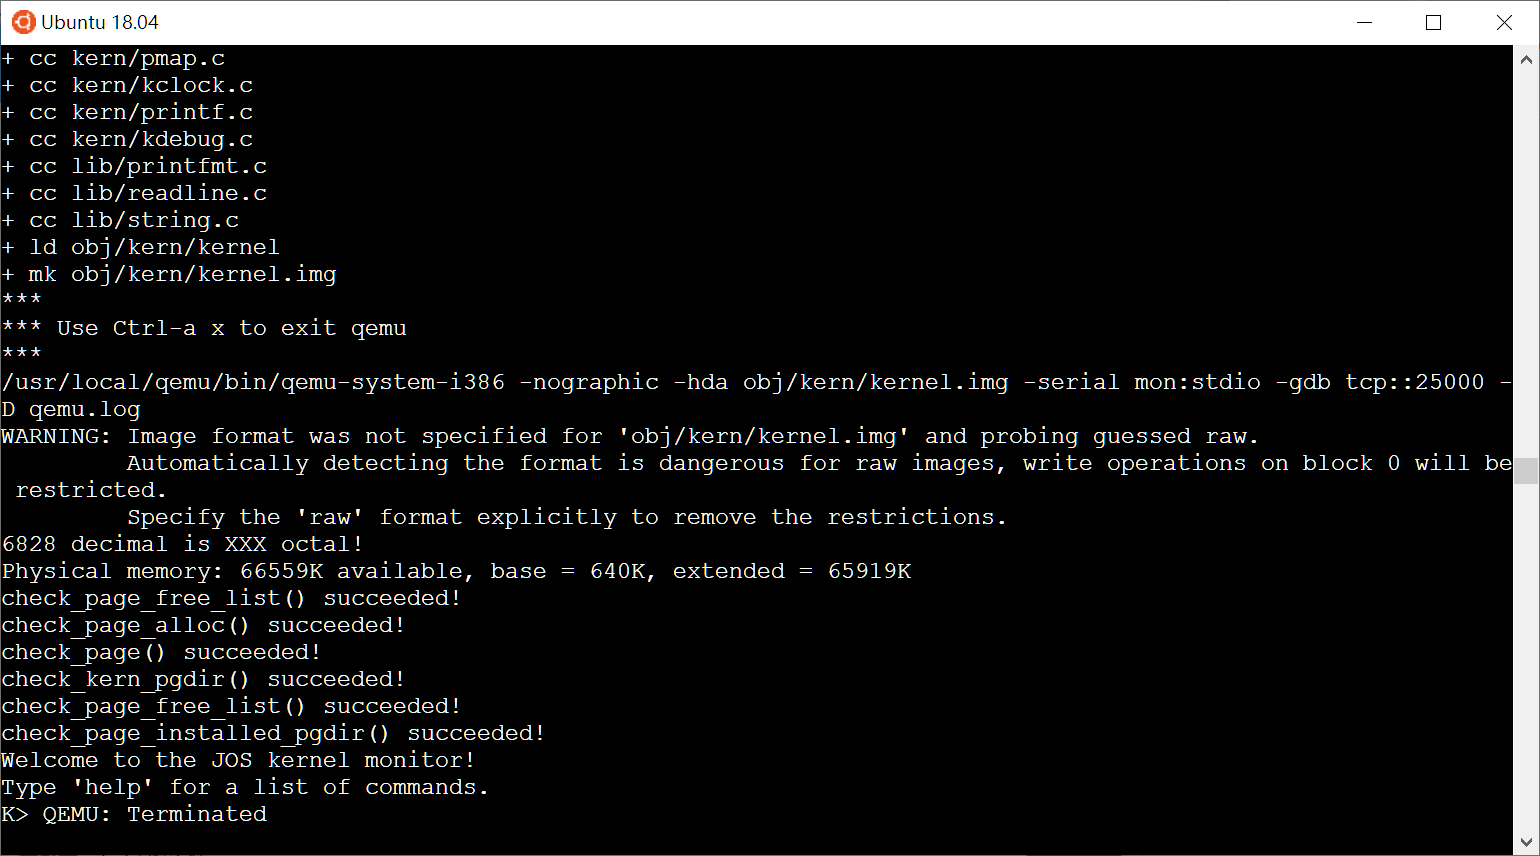
\includegraphics[width = .85\linewidth]{img/2.png}
        \caption{lab2实验结果-make qemu}
        \label{fig::figure2}
    \end{figure}

    \begin{figure}[H]
        \centering
        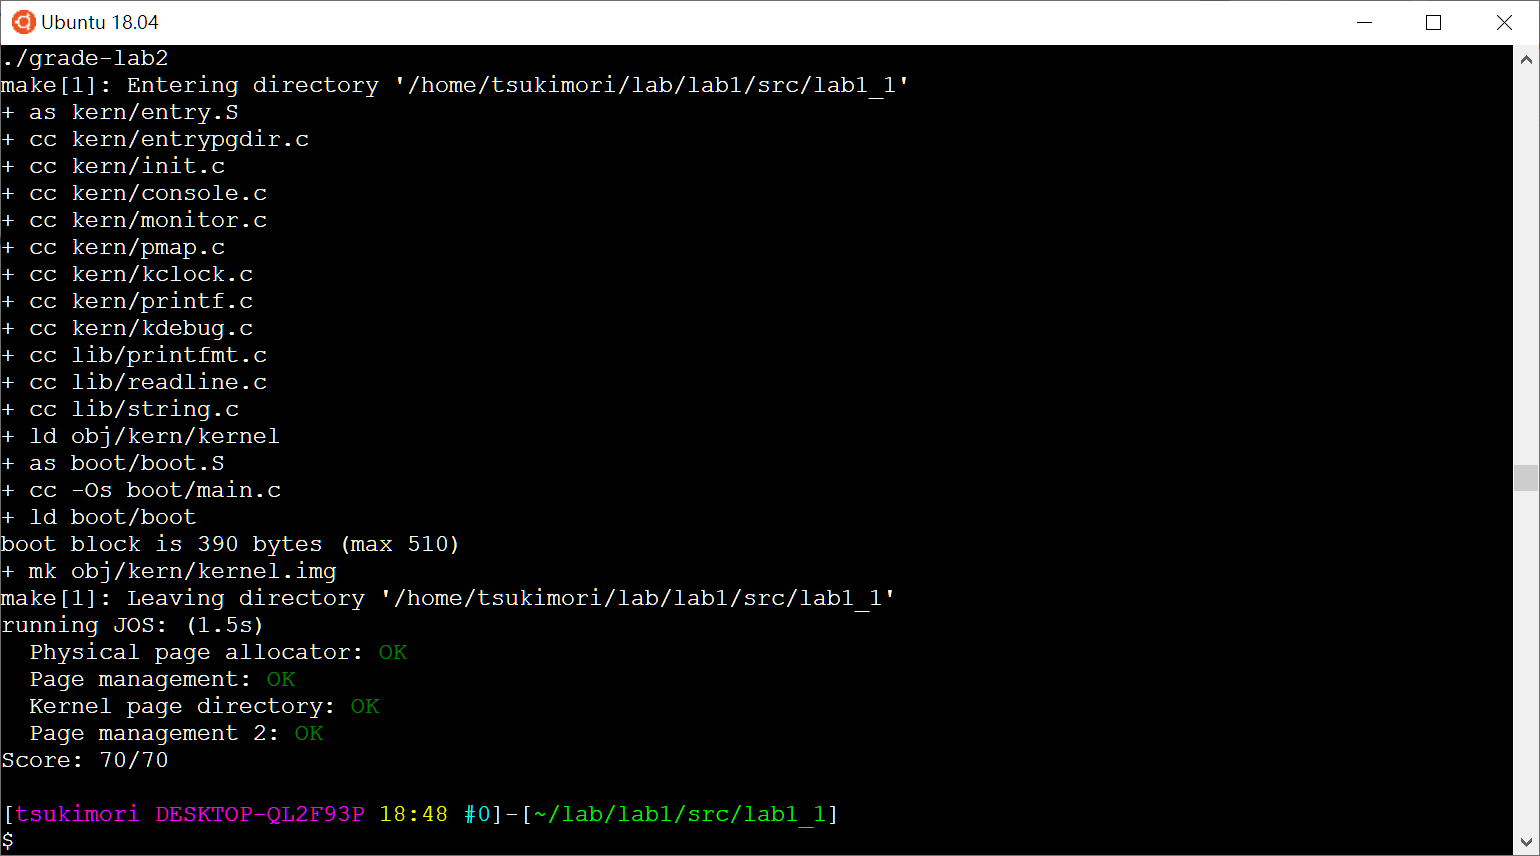
\includegraphics[width = .85\linewidth]{img/3.png}
        \caption{lab2实验结果-make grade}
        \label{fig::figure3}
    \end{figure}

\end{document}